\chapter{Уравнения, системы и неравенства}\label{chap:c11}\markright{Глава 12}
\begin{definition}\term{Корень уравнения} (\emph{root; solution of an equation}) — допустимое значение неизвестного, при котором равенство верно.\end{definition}
\begin{definition}\term{Решение неравенства} (\emph{solution of an inequality}) — значение неизвестного, при котором указанное сравнение верно.\end{definition}
\begin{definition}\term{Решение системы} (\emph{solution of a system}) — значения неизвестных, которые удовлетворяют всем её условиям одновременно.\end{definition}
\section{Линейные и квадратные уравнения}
\(ax + b = 0\) при \(a \ne  0\) имеет корень \(x = - \frac{b}{a}\). При \(a = 0,\allowbreak b = 0\) подходят все \(x\); при \(a = 0,\allowbreak b \ne  0\) решений нет.\par
\begin{definition}\term{Дискриминант} (\emph{discriminant}) квадратного уравнения \(ax^{2}+bx+c=0\) при \(a\ne0\) — число \(D=b^{2}-4ac\).\end{definition}
При \(D > 0\) два корня: \(x = \frac{- b \pm  \sqrt{D}}{2 a}\). При \(D = 0\) один корень: \(- \frac{b}{2 a}\). При \(D < 0\) действительных корней нет.\par
\section{Правила и проверка}
К обеим частям равенства или неравенства можно прибавить одно и то же выражение при сохранении ОДЗ.\par
При умножении или делении неравенства на отрицательное число знак меняется; на положительное — сохраняется.\par
Метод интервалов: отметь нули и запрещённые точки, определи знак на каждом участке и отдельно проверь включение границ.\par
При возведении уравнения в квадрат могут появиться посторонние корни: проверь найденные значения в исходном условии.\par
{\small\textit{Пример: \(- 2 x > 6\) даёт \(x < - 3\). Уравнение \(\sqrt{x + 2} = x\) требует \(x \ge  0\) ещё до возведения в квадрат.}}\par

% Дополнение к главе \ref{chap:c11}. Только действительные решения; формулы Кардано и Феррари не используются.
\subsection{Многочлены и уравнения третьей степени}
\begin{definition}
\term{Многочлен} (polynomial) от \(x\) — выражение
\[
P(x)=a_nx^n+a_{n-1}x^{n-1}+\cdots+a_1x+a_0.
\]
Если \(a_n\neq0\), число \(n\) называют \term{степенью многочлена} (degree). \term{Корень многочлена} (polynomial root) — число \(r\), для которого \(P(r)=0\).
\end{definition}

\begin{definition}
Корень \(r\) имеет \term{кратность} (multiplicity) \(k\), если \(P(x)=(x-r)^kQ(x)\), где \(Q(r)\neq0\). При \(k=1\) корень называют простым, при \(k>1\) — кратным.
\end{definition}

\begin{theorem}[Сумма и разность кубов]\label{thm:legacy-c11-1}
Для любых действительных \(a,b\)
\[
a^3-b^3=(a-b)(a^2+ab+b^2),\qquad
a^3+b^3=(a+b)(a^2-ab+b^2).
\]
\end{theorem}
\par\addvspace{5pt}\begin{lrbox}{\CatFlowBox}\begin{minipage}[t]{\linewidth}
\setlength{\parskip}{5pt}\setlength{\columnsep}{4.5mm}\setlength{\intextsep}{0pt}
\begin{wrapfigure}[11]{r}{54mm}

\includegraphics[width=54mm,height=58mm,keepaspectratio]{images/unique/art-192.png}
\label{catflow:192}
\end{wrapfigure}
\textit{Доказательство.} При раскрытии скобок в первом произведении получаем
\(a^3+a^2b+ab^2-a^2b-ab^2-b^3=a^3-b^3\).
Во втором произведении средние слагаемые также сокращаются:
\(a^3-a^2b+ab^2+a^2b-ab^2+b^3=a^3+b^3\).\hfill\(\blacksquare\)
\par\WFclear\end{minipage}\end{lrbox}%
\ifdim\dimexpr\ht\CatFlowBox+\dp\CatFlowBox\relax<64mm\dp\CatFlowBox=\dimexpr64mm-\ht\CatFlowBox\relax\fi%
\noindent\usebox{\CatFlowBox}\par\addvspace{5pt}


\begin{theorem}[Теорема Безу]\label{thm:legacy-c11-2}
\term{Теорема Безу} (factor theorem): для любого действительного \(r\) существует многочлен \(Q(x)\), для которого
\[
P(x)=(x-r)Q(x)+P(r).
\]
Следовательно, \(r\) — корень \(P\) тогда и только тогда, когда \(P(x)\) делится на \(x-r\) без остатка.
\end{theorem}
\begin{proof}
Для натурального \(k\)
\[
x^k-r^k=(x-r)(x^{k-1}+x^{k-2}r+\cdots+r^{k-1}).
\]
Равенство проверяется умножением: все промежуточные слагаемые сокращаются. Поэтому каждое слагаемое суммы \(P(x)-P(r)=\sum_{k=1}^n a_k(x^k-r^k)\) делится на \(x-r\). Это даёт нужный \(Q\). Если \(P(r)=0\), остаток равен нулю. Обратно, подставив \(x=r\) в \(P(x)=(x-r)Q(x)\), получаем \(P(r)=0\).
\end{proof}

\begin{theorem}[Рациональный корень]\label{thm:legacy-c11-3}
Пусть коэффициенты \(P(x)=a_nx^n+\cdots+a_0\) целые, \(a_n\neq0\), \(a_0\neq0\). Если \(\frac pq\) — \term{рациональный корень} (rational root), причём \(p,q\) взаимно просты и \(q>0\), то \(p\) делит \(a_0\), а \(q\) делит \(a_n\).
\end{theorem}
\par\addvspace{5pt}\begin{lrbox}{\CatFlowBox}\begin{minipage}[t]{\linewidth}
\setlength{\parskip}{5pt}\setlength{\columnsep}{4.5mm}\setlength{\intextsep}{0pt}
\begin{wrapfigure}[12]{r}{54mm}

\includegraphics[width=54mm,height=58mm,keepaspectratio]{images/unique/art-09.png}
\label{catflow:9}
\end{wrapfigure}
\textit{Доказательство.} Подстановка \(\frac pq\) и умножение на \(q^n\) дают
\[
a_np^n+a_{n-1}p^{n-1}q+\cdots+a_1pq^{n-1}+a_0q^n=0.
\]
Все слагаемые, кроме последнего, делятся на \(p\), поэтому \(p\) делит \(a_0q^n\). Поскольку \(p\) и \(q^n\) взаимно просты, \(p\) делит \(a_0\). Аналогично \(q\) делит \(a_np^n\), а значит, делит \(a_n\). Использованное свойство взаимной простоты следует из разложения на простые множители: множители делителя, отсутствующие в одном сомножителе, должны целиком входить в другой.\hfill\(\blacksquare\)
\par\WFclear\end{minipage}\end{lrbox}%
\ifdim\dimexpr\ht\CatFlowBox+\dp\CatFlowBox\relax<64mm\dp\CatFlowBox=\dimexpr64mm-\ht\CatFlowBox\relax\fi%
\noindent\usebox{\CatFlowBox}\par\addvspace{5pt}


Если старший коэффициент равен \(1\), рациональный корень может быть только целым делителем свободного члена. Проверяем кандидатов подстановкой, а найденный множитель \(x-r\) отделяем по теореме Безу. Если свободный член нулевой, сначала выносим \(x\). Отсутствие рациональных корней не означает отсутствия действительных: например, \(x^3-2=0\) имеет корень \(\sqrt[3]2\).

\begin{example}
Для \(P(x)=x^3-4x^2+x+6\) проверка даёт \(P(2)=0\). Поэтому
\[
P(x)=(x-2)(x^2-2x-3)=(x-2)(x-3)(x+1).
\]
Уравнение \(P(x)=0\) имеет корни \(-1,2,3\).
\end{example}

\begin{theorem}[Устранение квадратного слагаемого]\label{thm:legacy-c11-4}
В \term{кубическом уравнении} (cubic equation)
\(ax^3+bx^2+cx+d=0\), где \(a\neq0\), замена \(x=t-\frac{b}{3a}\) даёт \term{неполное кубическое уравнение} (depressed cubic)
\[
t^3+pt+q=0,\qquad
p=\frac{3ac-b^2}{3a^2},\qquad
q=\frac{2b^3-9abc+27a^2d}{27a^3}.
\]
\end{theorem}
\begin{proof}
После деления на \(a\) обозначим коэффициенты через \(B=\frac ba\), \(C=\frac ca\), \(D=\frac da\). Подставим \(x=t-\frac B3\) и раскроем скобки:
\[
\begin{aligned}
&\left(t-\frac B3\right)^3+B\left(t-\frac B3\right)^2+C\left(t-\frac B3\right)+D\\
&\qquad=t^3+\left(C-\frac{B^2}{3}\right)t+\frac{2B^3}{27}-\frac{BC}{3}+D.
\end{aligned}
\]
Коэффициент при \(t^2\) равен нулю. Подстановка \(B,C,D\) даёт указанные \(p,q\).
\end{proof}

Такая замена упрощает форму уравнения; сама по себе она не даёт готовой формулы корней. В задачах этого раздела после замены достаточно разложения на множители или выделения куба.

\subsection{Два вида уравнений четвёртой степени}
\begin{definition}
\term{Биквадратное уравнение} (biquadratic equation) имеет вид \(ax^4+bx^2+c=0\), где \(a\neq0\). Замена \(u=x^2\) приводит к квадратному уравнению \(au^2+bu+c=0\) с обязательным условием \(u\geq0\).
\end{definition}
Каждое \(u>0\) даёт два корня \(x=\pm\sqrt u\), значение \(u=0\) — один корень \(x=0\), а отрицательное \(u\) действительных корней не даёт.

\begin{example}
\(x^4-10x^2+9=0\) после замены \(u=x^2\) даёт \((u-1)(u-9)=0\). Поэтому \(x=-3,-1,1,3\).
\end{example}

\begin{definition}
\term{Возвратное уравнение четвёртой степени} (reciprocal quartic equation) в этом разделе — уравнение
\[
ax^4+bx^3+cx^2+bx+a=0,\qquad a\neq0,
\]
у которого коэффициенты симметричны относительно середины.
\end{definition}

\begin{theorem}[Замена для возвратного уравнения]\label{thm:legacy-c11-5}
Корни указанного возвратного уравнения ненулевые. Замена \(t=x+\frac1x\) сводит поиск действительных корней к
\[
at^2+bt+c-2a=0,\qquad |t|\geq2.
\]
Для каждого допустимого \(t\) решают \(x^2-tx+1=0\).
\end{theorem}
\par\addvspace{5pt}\begin{lrbox}{\CatFlowBox}\begin{minipage}[t]{\linewidth}
\setlength{\parskip}{5pt}\setlength{\columnsep}{4.5mm}\setlength{\intextsep}{0pt}
\begin{wrapfigure}[12]{l}{54mm}

\includegraphics[width=54mm,height=58mm,keepaspectratio]{images/unique/art-24.png}
\label{catflow:24}
\end{wrapfigure}
\textit{Доказательство.} При \(x=0\) левая часть исходного уравнения равна \(a\neq0\), поэтому деление на \(x^2\) допустимо. Получаем
\[
a\left(x^2+\frac1{x^2}\right)+b\left(x+\frac1x\right)+c=0.
\]
Из \(t=x+\frac1x\) следует \(x^2+\frac1{x^2}=t^2-2\), что даёт квадратное уравнение для \(t\). Обратная подстановка равносильна \(x^2-tx+1=0\). Его дискриминант \(t^2-4\) неотрицателен ровно при \(|t|\geq2\); свободный член \(1\) исключает нулевой корень. Значит, указанное условие необходимо и достаточно.\hfill\(\blacksquare\)
\par\WFclear\end{minipage}\end{lrbox}%
\ifdim\dimexpr\ht\CatFlowBox+\dp\CatFlowBox\relax<64mm\dp\CatFlowBox=\dimexpr64mm-\ht\CatFlowBox\relax\fi%
\noindent\usebox{\CatFlowBox}\par\addvspace{5pt}


\begin{example}
Для \(x^4-3x^3+2x^2-3x+1=0\) получаем \(t^2-3t=0\), то есть \(t=0\) или \(t=3\). Значение \(t=0\) не удовлетворяет \(|t|\geq2\). При \(t=3\) имеем \(x^2-3x+1=0\), откуда
\[
x=\frac{3-\sqrt5}{2}\quad\text{или}\quad x=\frac{3+\sqrt5}{2}.
\]
\end{example}

\Needspace{7\baselineskip}\section*{Задачи}
\begingroup\setlength{\parskip}{2pt}
\noindent\begin{minipage}[t]{\linewidth}\textbf{12.1.} Реши \(3 x - 7 = 11\).\par\end{minipage}\par
\noindent\begin{minipage}[t]{\linewidth}\textbf{12.2.} Реши \(2 (x - 3) = 5 x + 9\).\par\end{minipage}\par
\noindent\begin{minipage}[t]{\linewidth}\textbf{12.3.} Реши \(x^{2} - 5 x + 6 = 0\).\par\end{minipage}\par
\noindent\begin{minipage}[t]{\linewidth}\textbf{12.4.} Реши \(2 x^{2} - 8 = 0\).\par\end{minipage}\par
\noindent\begin{minipage}[t]{\linewidth}\textbf{12.5.} Реши \(\dfrac{x + 1}{x - 2} = 2\).\par\end{minipage}\par
\noindent\begin{minipage}[t]{\linewidth}\textbf{12.6.} Реши систему: \(x + y = 7;\allowbreak x - y = 1\).\par\end{minipage}\par
\par\addvspace{5pt}\begin{lrbox}{\CatFlowBox}\begin{minipage}[t]{\linewidth}
\setlength{\parskip}{5pt}\setlength{\columnsep}{4.5mm}\setlength{\intextsep}{0pt}
\begin{wrapfigure}[12]{r}{54mm}

\includegraphics[width=54mm,height=58mm,keepaspectratio]{images/unique/art-39.png}
\label{catflow:39}
\end{wrapfigure}
\textbf{12.7.} Реши \(- 3 x > 12\).\par

\textbf{12.8.} Реши \(x^{2} - 9 \le  0\).\par

\textbf{12.9.} Реши \((x - 1) (x + 2) > 0\).\par

\textbf{12.10.} Реши \(\dfrac{x - 3}{x + 1} \le  0\).\par

\textbf{12.11.} Реши \(| 2 x - 1 | = 5\).\par

\textbf{12.12.} Реши \(\sqrt{x + 2} = x\).\par

\textbf{12.13.} Поездка на такси стоит \(150\) рублей за подачу и \(30\) рублей за километр. Счёт составил \(510\) рублей. Какое расстояние проехали?\par
\par\WFclear\end{minipage}\end{lrbox}%
\ifdim\dimexpr\ht\CatFlowBox+\dp\CatFlowBox\relax<64mm\dp\CatFlowBox=\dimexpr64mm-\ht\CatFlowBox\relax\fi%
\noindent\usebox{\CatFlowBox}\par\addvspace{5pt}

\noindent\begin{minipage}[t]{\linewidth}\textbf{12.14.} За \(3\) одинаковых блокнота и ручку стоимостью \(80\) рублей заплатили \(440\) рублей. Сколько стоит блокнот?\par\end{minipage}\par
\noindent\begin{minipage}[t]{\linewidth}\textbf{12.15.} Для покупки билетов по \(350\) рублей выделено \(2000\) рублей. Какое максимальное целое число билетов можно купить?\par\end{minipage}\par
\noindent\begin{minipage}[t]{\linewidth}\textbf{12.16.}\starmark{} Реши \(\sqrt{2 x + 3} = x\).\par\end{minipage}\par
\noindent\begin{minipage}[t]{\linewidth}\textbf{12.17.}\starmark{} Реши \(\dfrac{x - 2}{x + 3} \ge  1\).\par\end{minipage}\par
\noindent\begin{minipage}[t]{\linewidth}\textbf{12.18.}\starmark{} У прямоугольного участка периметр \(34\) м, площадь \(60\) м\(^{2}\). Найди стороны.\par\end{minipage}\par
\noindent\begin{minipage}[t]{\linewidth}\textbf{12.19.} Докажите формулы Виета: если \(x_1,x_2\) — действительные корни \(ax^2+bx+c=0\), \(a\neq0\), с учётом кратности, то \(x_1+x_2=-\dfrac ba\), \(x_1x_2=\dfrac ca\).\par\end{minipage}\par
\noindent\begin{minipage}[t]{\linewidth}\textbf{12.20.} Докажите, что квадратное уравнение \(ax^2+bx+c=0\), \(a\neq0\), имеет действительный корень тогда и только тогда, когда \(D=b^2-4ac\geq0\). Используйте выделение полного квадрата.\par\end{minipage}\par
\noindent\begin{minipage}[t]{\linewidth}\textbf{12.21.} Решите в действительных числах \(x^3-8=0\), разложив разность кубов на множители.\par\end{minipage}\par
\noindent\begin{minipage}[t]{\linewidth}\textbf{12.22.} Решите в действительных числах \(x^3+27=0\), разложив сумму кубов на множители.\par\end{minipage}\par
\noindent\begin{minipage}[t]{\linewidth}\textbf{12.23.} Решите \(x^3-6x^2+11x-6=0\). Найдите целый корень, затем выделите соответствующий линейный множитель.\par\end{minipage}\par
\noindent\begin{minipage}[t]{\linewidth}\textbf{12.24.} Решите \(2x^3-3x^2-8x+12=0\) в действительных числах.\par\end{minipage}\par
\noindent\begin{minipage}[t]{\linewidth}\textbf{12.25.}\starmark{} В уравнении \(x^3-6x^2+9x-4=0\) сделайте замену \(x=t+2\). Решите полученное уравнение и вернитесь к \(x\).\par\end{minipage}\par
\noindent\begin{minipage}[t]{\linewidth}\textbf{12.26.} Решите биквадратное уравнение \(x^4-5x^2+4=0\).\par\end{minipage}\par
\noindent\begin{minipage}[t]{\linewidth}\textbf{12.27.} Решите в действительных числах \(x^4+3x^2-4=0\), проверив допустимость найденных значений \(x^2\).\par\end{minipage}\par
\noindent\begin{minipage}[t]{\linewidth}\textbf{12.28.}\starmark{} Решите возвратное уравнение \(x^4-5x^3+6x^2-5x+1=0\). Для каждого корня уравнения относительно \(t=x+\dfrac1x\) проверьте условие \(|t|\geq2\).\par\end{minipage}\par
\par\Needspace{12\baselineskip}\section*{Олимпиадные задачи}
\par\addvspace{2pt}\begin{lrbox}{\CatFlowBox}\begin{minipage}[t]{\linewidth}
\setlength{\parskip}{2pt}\setlength{\columnsep}{4.5mm}\setlength{\intextsep}{0pt}
\begin{wrapfigure}[11]{l}{54mm}
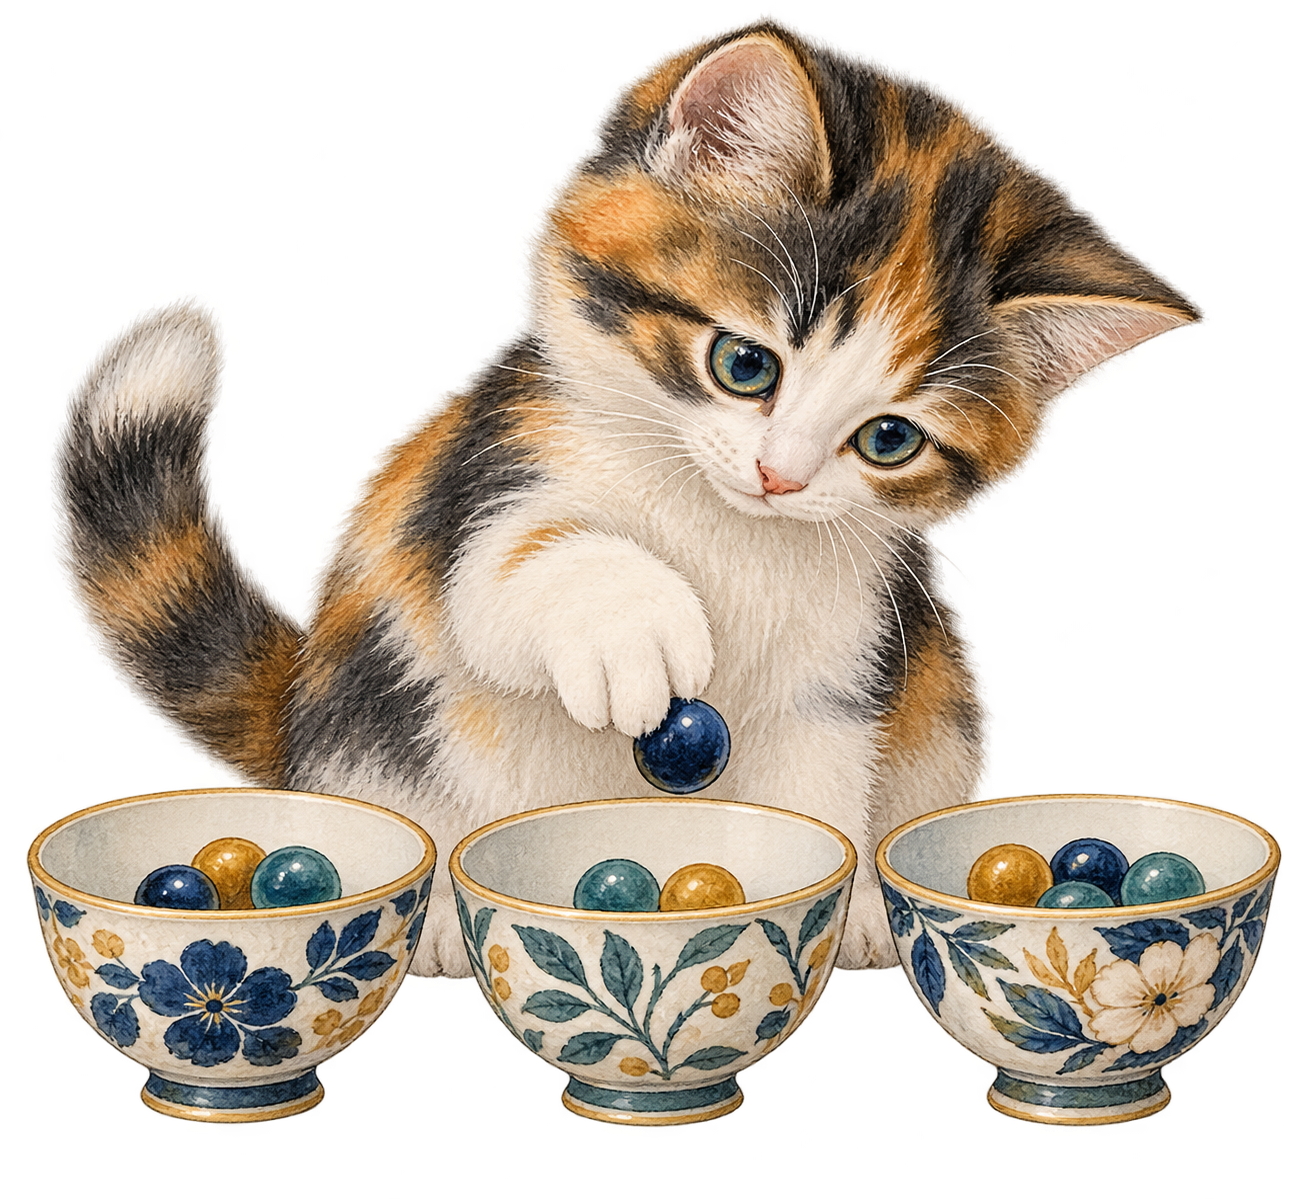
\includegraphics[width=54mm,height=58mm,keepaspectratio]{images/unique/art-299.png}
\label{catflow:299}
\end{wrapfigure}
\textbf{12.29.} {\small\itshape\href{https://mmo.mccme.ru/books/mmo-35-57.pdf}{ММО, 1935, II тур, серия B, № 1}; редакция условия.}\par Сколько действительных троек удовлетворяет \(x+y=2\), \(xy-z^2=1\)? Найди их.\par

\textbf{12.30.}\starmark{} {\small\itshape\href{https://mmo.mccme.ru/books/mmo-35-57.pdf}{ММО, 1937, I тур, № 1}; редакция условия.}\par Для действительного \(a\) реши над \(\mathbb R\) систему \[\begin{aligned}x+y+z&=a,\\x^2+y^2+z^2&=a^2,\\x^3+y^3+z^3&=a^3.\end{aligned}\]\par
\par\WFclear\end{minipage}\end{lrbox}%
\ifdim\dimexpr\ht\CatFlowBox+\dp\CatFlowBox\relax<58mm\dp\CatFlowBox=\dimexpr58mm-\ht\CatFlowBox\relax\fi%
\noindent\usebox{\CatFlowBox}\par\addvspace{2pt}

\endgroup
